\section{Experiments}
\label{sec:experiments}

In this section we present experiments corroborating our theoretical analysis (\Secref{sec:analysis}).
The latter establishes that, under certain conditions, a linear RNN with state space dimension~$d$ extrapolates when learning from a teacher network with state space dimension~\smash{$\hat{d}$} via training sequences of length~$k$, irrespective of how large~$d$ is compared to \smash{$\hat{d}$} and~$k$. %\amirg{this sentence isn't clear. I suggest dropping everything starting at "irrespective"}
A key condition underlying the result is that $k$ is larger than $2 \hat{d}$.
\Secref{sec:exp:sym_teacher} below considers the theoretically analyzed setting, and empirically evaluates extrapolation as~$k$ varies.
Its results demonstrate a phase transition, in the sense that extrapolation takes place when \smash{$k > 2 \hat{d}$}, in compliance with theory, but on the other hand fails when $k$ falls below~\smash{$2 \hat{d}$}, in which case the theory indeed does not guarantee extrapolation.
\Secref{sec:exp:step_func} displays the same phenomenon with linear RNNs that do not adhere to some of the assumptions made by the theory (in particular the assumption of symmetric transition matrices, and those concerning balancedness).
Finally, \Secref{sec:exp:non_linear_teacher} considers non-linear RNNs (specifically, Gated Recurrent Unit networks \cite{chung2014empirical}), and shows that they too exhibit a phase transition in extrapolation as the training sequence length varies.
For brevity, we defer some of the details of our implementation, as well as additional experiments, to \Appref{sec:apdx:additional_experiments}.

\subsection{Theoretically Analyzed Setting} \label{sec:exp:sym_teacher}

Our first experiment considers the setting described in \Secref{sec:setup} and theoretically analyzed in \Secref{sec:analysis}.
As representative values for the state space dimensions of the teacher and (overparameterized) student, we choose \smash{$\hat{d} = 5$} and $d = 40$ respectively (higher state space dimensions for the student, namely $d = 100$ and $d = 200$, yielded qualitatively identical results).
For a given training sequence length~$k$, the student is learned via GD applied directly to the population loss defined in \Eqref{eq:population_loss} (applying GD to the empirical loss defined in \Eqref{eq:empirical_loss}, with $N = 10,000$ training examples, led to similar results). %\amirg{isn't this covered in the next section? Why mention it here?}\nadav{the rationale was that next section treats a different setting}).
\Figref{fig:phase_transition_v2}(a) reports the extrapolation error (quantified by the $\ell_\infty$ distance between the impulse response of the learned student and that of the teacher) as a function of~$k$.
As can be seen, extrapolation exhibits a phase transition that accords with our theory: when \smash{$k > 2 \hat{d}$} extrapolation error is low, whereas when $k$ falls below~\smash{$2 \hat{d}$} extrapolation error is high.

\subsection{Other Settings With Linear Recurrent Neural Networks} \label{sec:exp:step_func}

To assess the generality of our findings, we experiment with linear RNNs in settings that do not adhere to some of the assumptions made by our theory.
Specifically, we evaluate settings in which:
\emph{(i)}~the teacher is unbalanced, meaning \smash{$\hat{\mB} \neq \hat{\mC}^\top$}, and its transition matrix~\smash{$\hat{\mA}$} is non-symmetric;
\emph{(ii)}~the student's transition matrix~$\mA$ is not restricted to be symmetric;
\emph{(iii)}~learning is implemented by optimizing the empirical loss defined in \Eqref{eq:empirical_loss} (rather than the population loss defined in \Eqref{eq:population_loss});
and
\emph{(iv)}~optimization is based on Adam \cite{kingma2014adam} (rather than GD), emanating from standard near-zero initialization which is generally unbalanced (namely, $\mB\neq \mC^\top$).
\Figref{fig:phase_transition_v2}(b) reports the results of an experiment where the state space dimensions of the teacher and (overparameterized) student are \smash{$\hat{d} = 10$} and $d = 50$ respectively (higher state space dimensions for the student, namely $d = 100$ and $d = 200$, yielded qualitatively identical results), and where the teacher implements a delay line of \smash{$\hat{d}$} time steps (for details see \Appref{sec:apdx:unbalanced_teacher_generation}).
Similar results obtained with randomly generated teachers are reported in \Appref{sec:apdx:additional_experiments}.
As can be seen, despite the fact that our theory does not apply to the evaluated settings, its conclusions still hold~---~extrapolation error is low when the training sequence length~$k$ is greater than~\smash{$2 \hat{d}$}, and high when $k$ falls below~\smash{$2 \hat{d}$}.

\begin{figure}[H]
    \centering
    \subfigure[Theoretically analyzed setting]{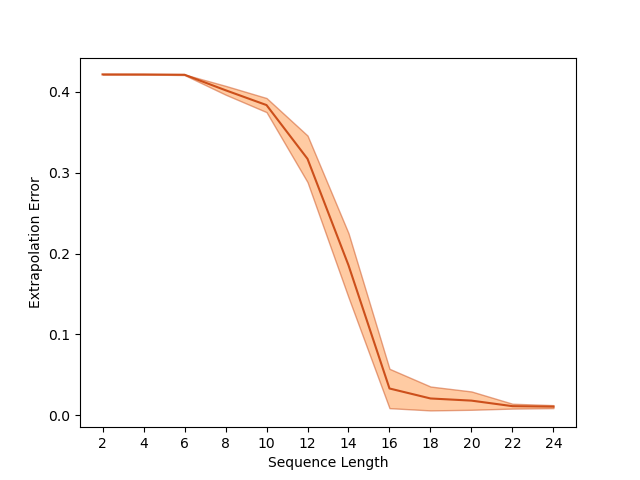
\includegraphics[width=0.45\textwidth,height=3.6cm]{figures/extrapolation_as_func_of_k_theoretical_setup.png}}
    \subfigure[Other setting with linear RNN]{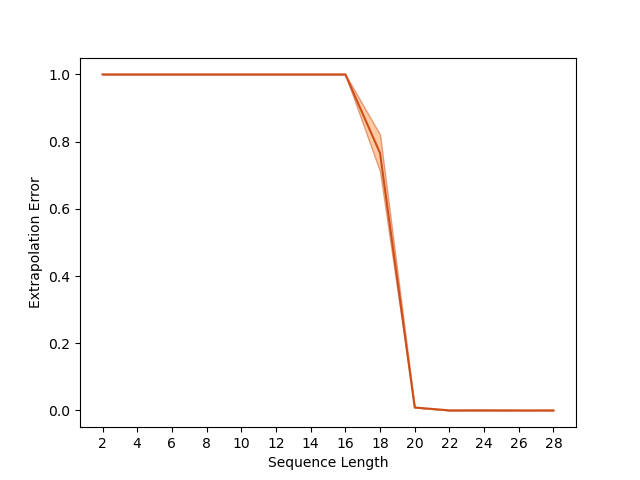
\includegraphics[width=0.45\textwidth,height=3.6cm]{figures/extrapolation_as_func_of_k_step_func_init_1e-06_v2.png}} 
    \caption{
    Demonstration of implicit extrapolation with linear RNNs.
    Plots show extrapolation error (average over three random seeds, with shaded region marking standard deviation) as a function of training sequence length~$k$, for a student with state space dimension~$d$ learning from a teacher with state space dimension~\smash{$\hat{d}$}, where \smash{$d \gg \hat{d}$}.
    (a) Models adhere to the setting described in \Secref{sec:setup} and theoretically analyzed in \Secref{sec:analysis}, with \smash{$\hat{d} = 5$}, $d = 40$.
    (b) Models do not adhere to some of the assumptions made by the theory, and \smash{$\hat{d} = 10$}, $d = 50$.
    Notice that extrapolation exhibits a phase transition that accords with theory~---~when \smash{$k > 2 \hat{d}$} extrapolation error is low, and when $k$ falls below~\smash{$2 \hat{d}$} extrapolation error is high.
    For further details see Sections \ref{sec:exp:sym_teacher} and~\ref{sec:exp:step_func} and \Appref{sec:apdx:additional_experiments}.
    }
    \label{fig:phase_transition_v2}
\end{figure}

\subsection{Non-Linear Recurrent Neural Networks} \label{sec:exp:non_linear_teacher}

As a final experiment, we explore implicit extrapolation with non-linear RNNs, namely GRU networks.
Specifically, we evaluate the extent to which a student GRU with state space dimension $d_g = 100$ extrapolates when learning from a teacher GRU with state space dimension \smash{$\hat{d}_g = 10$} (higher state space dimensions for the student, namely $d_g = 200$ and $d_g = 500$, yielded qualitatively identical results).
The student is learned by optimizing an empirical loss comprising training sequences of length~$k_g$, where $k_g$ is predetermined.
Optimization is based on Adam emanating from standard near-zero initialization.
\figref{fig:gru_extrapolation}(a) reports the extrapolation error (quantified by the $\ell_\infty$ distance between the response of the learned student and that of the teacher, averaged across randomly generated input sequences) for different choices of~$k_g$.
As can be seen, similarly to the case with linear RNNs (see Sections \ref{sec:exp:sym_teacher} and~\ref{sec:exp:step_func}), there exists a critical threshold for the training sequence length~$k_g$, above which extrapolation error is low and below which extrapolation error is high.\footnote{%
Note that this critical threshold is around four times the teacher's state space dimension, whereas with linear RNNs the critical threshold was around two times the teacher's state space dimension.
Theoretically explaining this difference is viewed as an interesting direction for future work.
}
%\amirg{I'm not sure we want to show the impulse response for the GRU. It's not even clear what that is? Is it the response to an impulse? If yes, we shoudld explain, and should also say that our theory doesn't say that the first $k$ impulse points should be recovered in this case. We can perhaps turn it into an advantage by saying that it's interesting to study.}
\figref{fig:gru_extrapolation}(b) displays the average output response over different inputs of the teacher alongside those of two students~---~one trained with sequences of length $k_g = 30$, and the other with sequences of length $k_g = 60$.\footnote{%
Note that with GRU networks, in contrast to linear RNNs, the impulse response does not identify the input-output mapping realized by a network.
It is presented in \figref{fig:gru_extrapolation}(b) for demonstrative purposes.
}
As expected, the impulse response of each student tracks that of the teacher for the first $k_g$ time steps (where $k_g$ is student-dependent).
However, while the student for which $k_g = 30$ fails to track the teacher beyond $k_g$ time steps, the student for which $k_g = 60$ succeeds, thereby exemplifying implicit extrapolation. %This behavior resembles the one of linear RNNs, where below a certain $k$ no extrapolation occurs but above it we do see it.

\begin{figure}
\centering
\subfigure[Extrapolation vs.~training sequence length]
{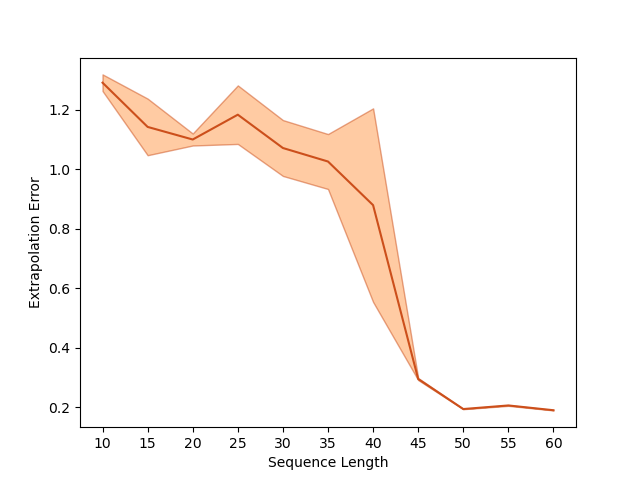
\includegraphics[width=0.45\textwidth,height=3.6cm]{figures/extrapolation_as_func_of_k_gru.png}}
\subfigure[Average output over several inputs]
{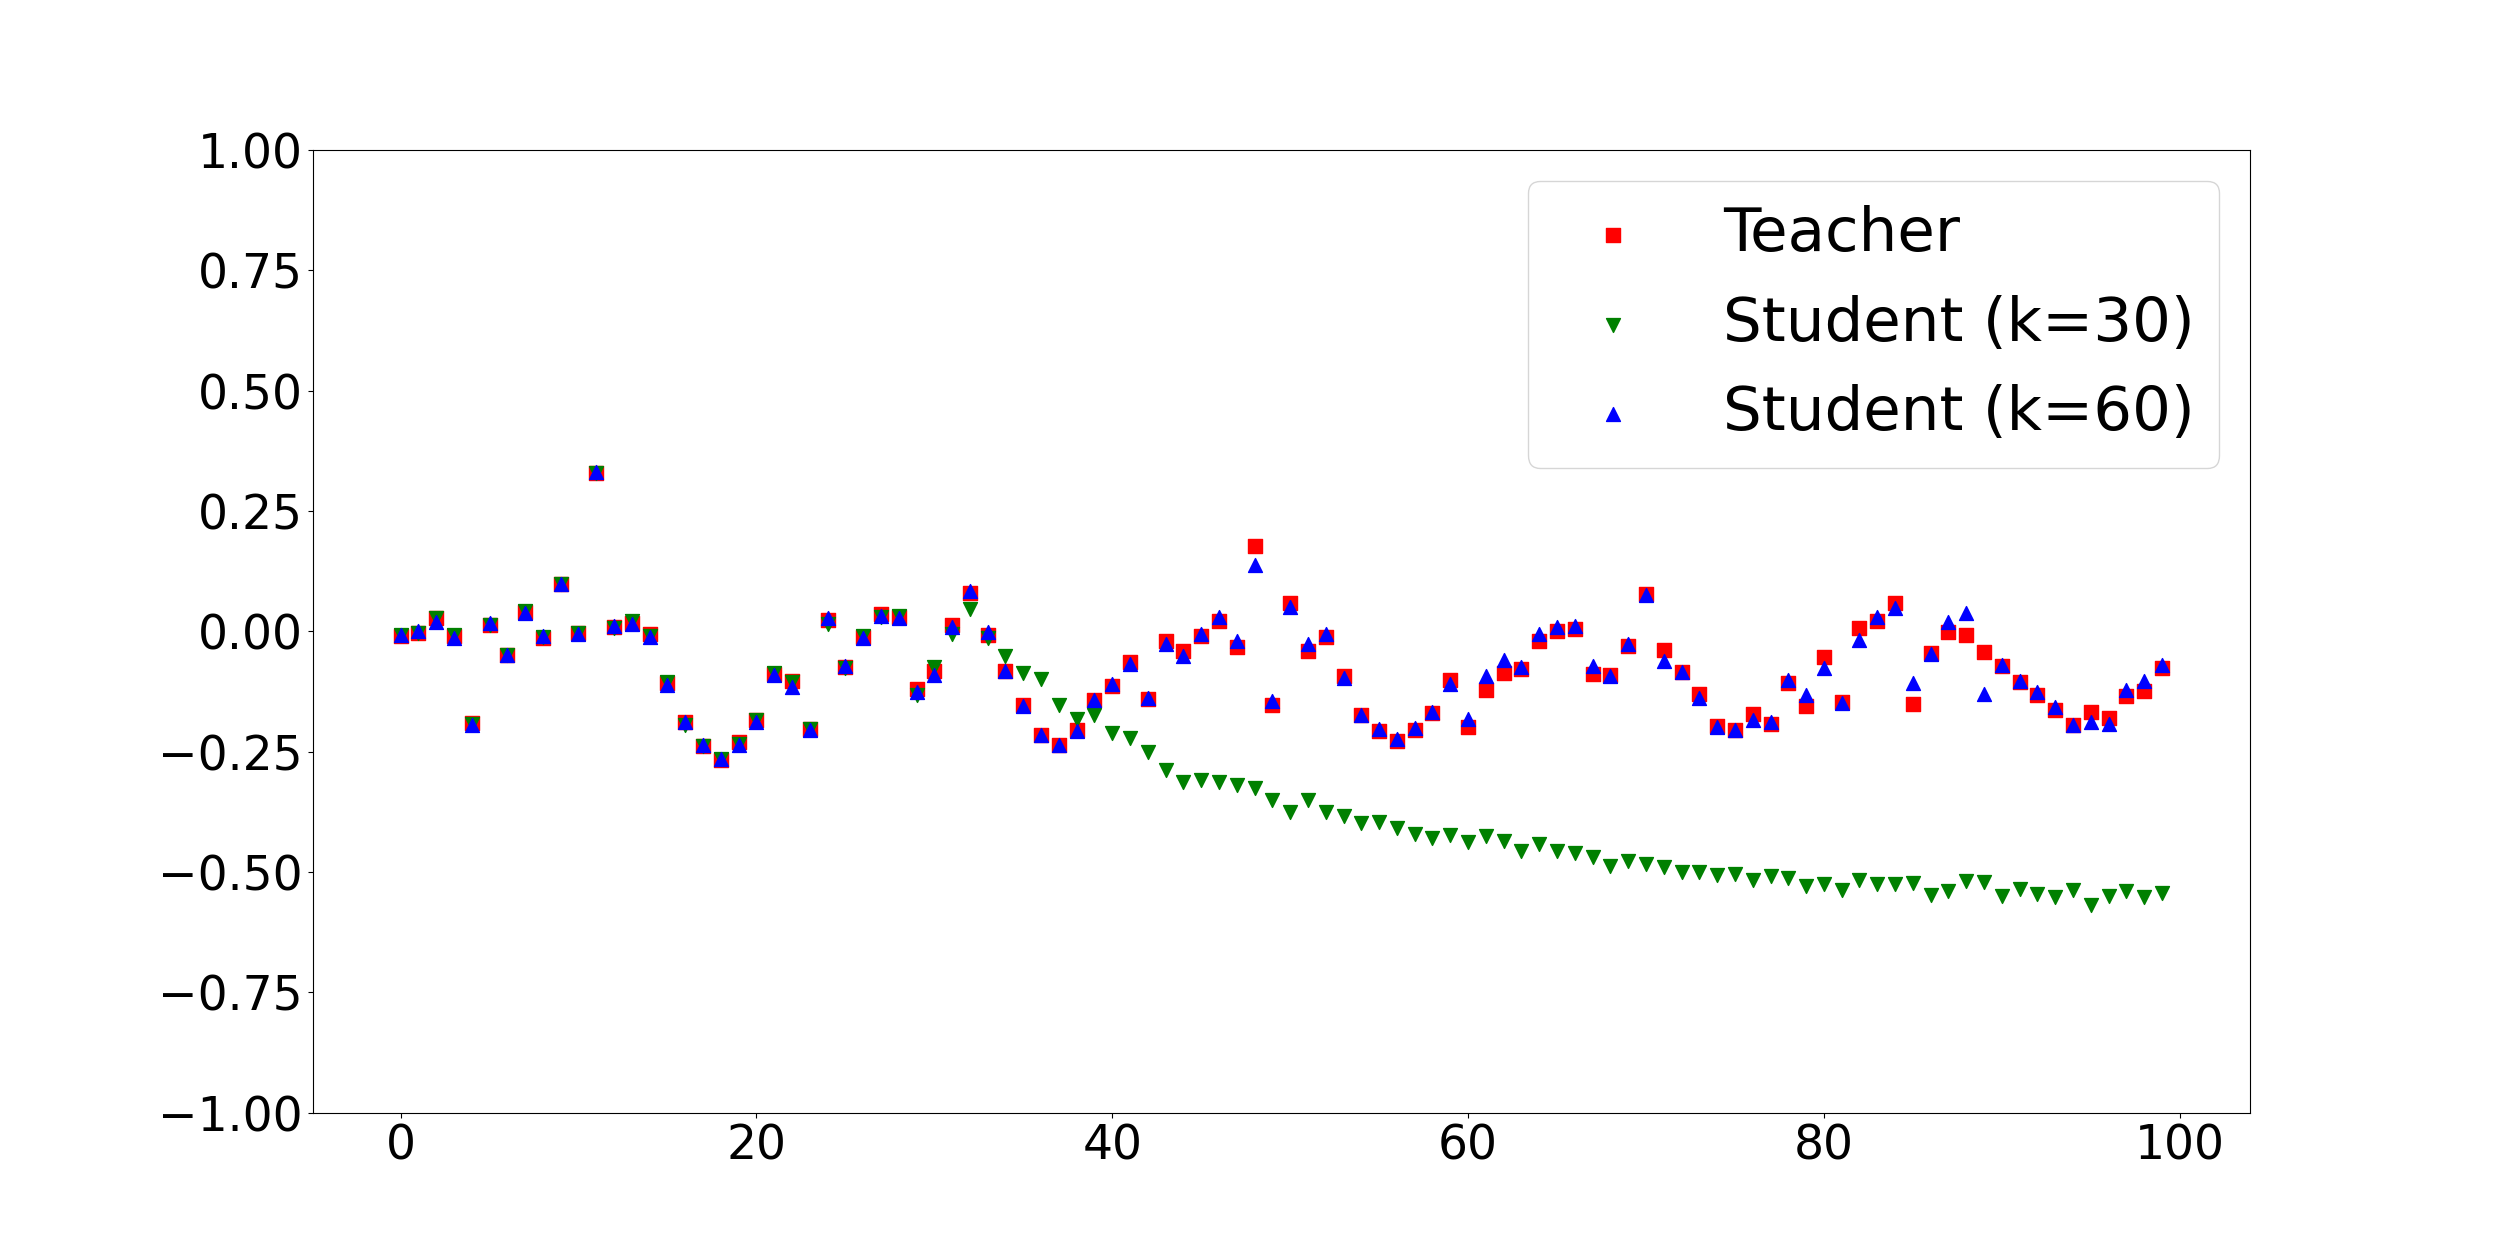
\includegraphics[width=0.52\textwidth,height=3.6cm]{figures/gru_impulse_responses.png}}
\caption{
Demonstration of implicit extrapolation with non-linear RNNs, namely GRU networks.
Plots show results for a student with state space dimension $d_g = 100$ learning from a teacher with state space dimension \smash{$\hat{d}_g = 10$} using training sequences of length~$k_g$, where $k_g$ varies.
(a)~Extrapolation error (average over ten random seeds, with shaded region marking standard deviation) as a function of~$k_g$.
(b)~Average output over several inputs of teacher and student for different choices of~$k_g$.
Notice that, similarly to the case with linear RNNs, there exists a critical threshold for~$k_g$ above which extrapolation error is low and below which extrapolation error is high.
See more details  in \Appref{sec:apdx:additional_experiments}.
}
\label{fig:gru_extrapolation}
\end{figure}